\section{Metodología}
\label{sec:metodologia}

\subsection{Datos, modelo SEVARTI y preparación}
\label{sec:3.1}

Trabajamos con una base PostgreSQL del Observatorio Canguro a la que accedimos en modo de solo lectura. Para organizar la información longitudinal adoptamos SEVARTI (Stages--Episodes--Variables--Topics of Interest), el modelo conceptual facilitado por la Fundación Canguro \cite{r4}. Allí las etapas corresponden a momentos del seguimiento; los episodios representan eventos como hospitalización o posición canguro; las variables contienen las mediciones, y los tópicos de interés permiten estudiar preguntas clínicas. Con esta organización podemos relacionar cada dato con el niño, la visita y el contexto en que se registró (Figura~\ref{fig:1}).

\begin{figure}[t]
\centering
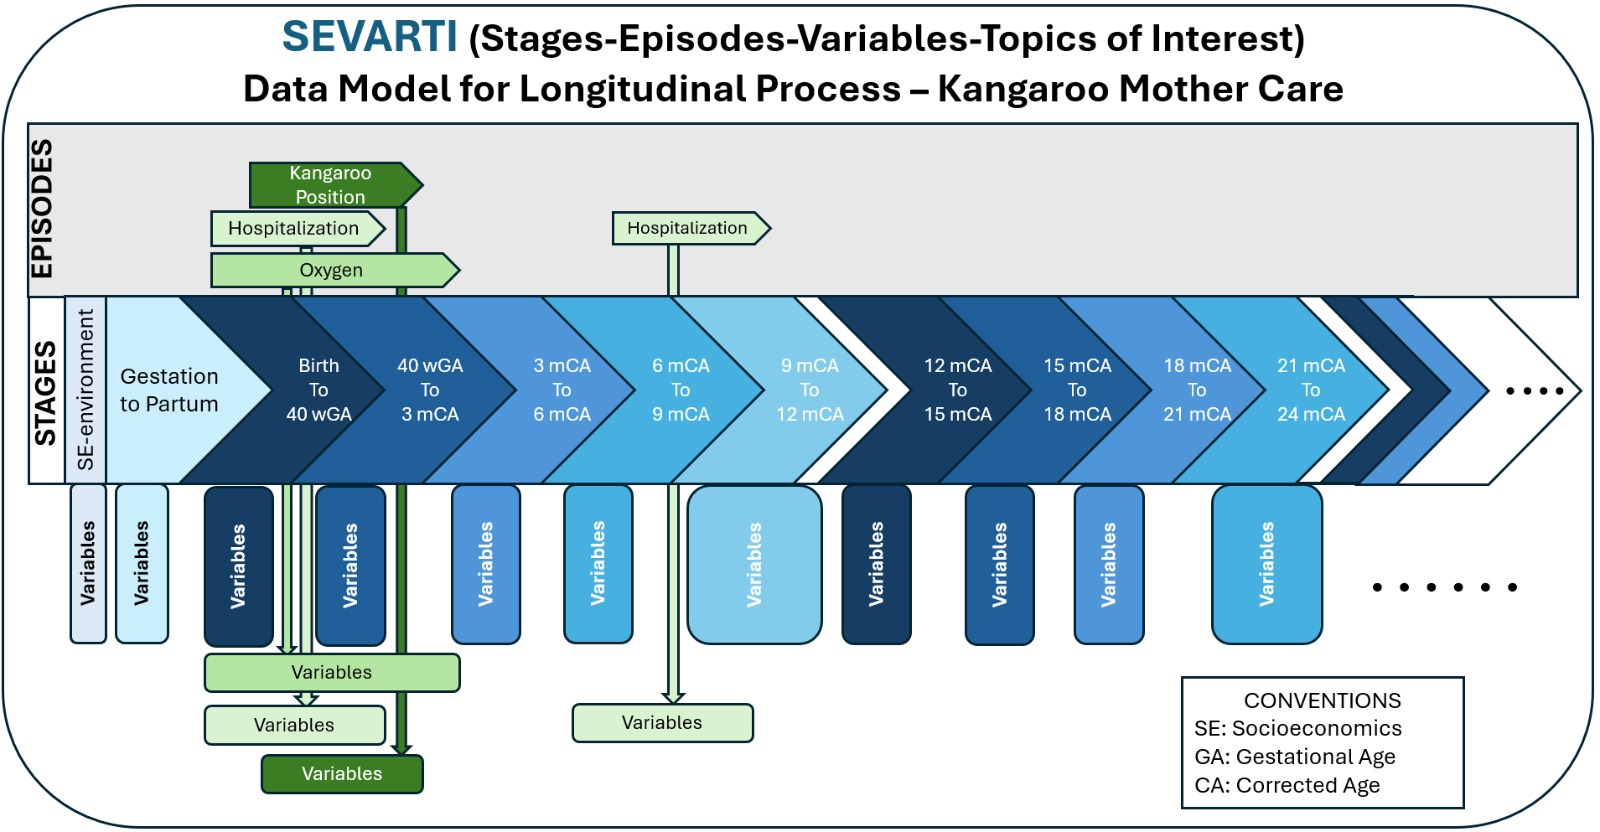
\includegraphics[width=\columnwidth]{figuras/image1.jpeg}
\caption{Modelo conceptual SEVARTI: etapas, episodios y variables vinculados al seguimiento. \fuente{Fundación Canguro, figura institucional facilitada para este estudio \cite{r4}.}}
\label{fig:1}
\end{figure}

La base original no sigue directamente la estructura SEVARTI, por eso construimos un adaptador que reúne los registros en seis entidades: esquema de variables, etapas, sujetos, mediciones, episodios y cambios conocidos en los sistemas de registro. El diccionario de variables, que pueden revisar los expertos, indica las unidades, los códigos de ausencia y las reglas de validez. Así evitamos programar reglas distintas para cada variable y podemos mantener el sistema cuando cambia la información disponible.

Para comparar las mediciones a lo largo del seguimiento usamos la edad corregida (EC), calculada a partir de la edad gestacional al nacer (EG). La Ecuación~(\ref{eq:1}) muestra el cálculo en días. Conservamos las fechas reales de las visitas, porque son necesarias para comprobar en qué momento se conocía cada dato.

\begin{equation}
\text{EC (días)} = \text{edad posnatal (días)} - 7\,(40-\text{EG})
\label{eq:1}
\end{equation}

En el corte analizado, cerca del 76 \% de las mediciones no tenía una ubicación temporal explícita. Cuando la fecha, la etapa y la edad registrada eran coherentes, el adaptador permitió reconstruir su posición en el seguimiento. Los valores faltantes se conservaron como tales y se identificaron códigos especiales, unidades incorrectas y registros incompatibles. También tuvimos en cuenta el cambio del sistema de captura ocurrido en 2022, ya que modificó patrones de registro importantes para la evaluación temporal.

Decidimos no completar automáticamente los valores faltantes ni modificar la base de origen. En lugar de ello, identificamos los registros que no debían utilizarse para aprender un valor y dejamos su ausencia explícita cuando otras estimaciones los necesitaban. Esta decisión buscó evitar que la limpieza ocultara problemas reales. La máscara de exclusión quedó versionada y afectó al 1,6 \% de 3,53 millones de datos numéricos; el 52 \% de esas exclusiones correspondió a códigos especiales.

\subsection{Etapa 1: detección y revisión de anomalías}
\label{sec:3.2}

La primera etapa de KMCPred examina cada medición desde cinco puntos de vista. Primero comprueba que su tipo, unidad y fecha sean posibles. Después busca valores inusuales, teniendo en cuenta códigos especiales y posibles errores de unidad. En el tercer nivel compara la medición con lo esperado para un niño con antecedentes similares mediante LightGBM cuantílico; el modelo no recibe como entrada el propio valor que intenta revisar. El cuarto nivel contrasta la trayectoria entre visitas y el quinto busca cambios persistentes por trimestre en residuos, datos faltantes o redondeos, utilizando CUSUM \cite{r12,r13,r14,r15,r16,r17,r25,r26}.

Para identificar valores poco habituales utilizamos medidas estadísticas robustas y tres cuantiles esperados (0,25; 0,50 y 0,75). Cuando hay suficientes datos de calibración (al menos 1/$\alpha$, es decir, 20 con el umbral $\alpha$ = 0,05 de producción), aplicamos un criterio conformal de p $\leq$ 0,05. Su objetivo es limitar las alertas sobre datos normales bajo las condiciones de calibración, aunque no garantiza que todas las alertas correspondan a errores. El sistema conserva el dato original y explica por qué debe revisarse; solo los registros claramente inconsistentes se excluyen como objetivos de aprendizaje, sin eliminar al niño completo.

Para identificar valores que se alejan considerablemente del comportamiento habitual de una variable, utilizamos una medida estadística robusta basada en la mediana y la desviación absoluta mediana (MAD). La MAD se multiplica por 1,4826 para obtener una escala comparable con la desviación estándar cuando los datos siguen aproximadamente una distribución normal \cite{r27}. Siguiendo el criterio propuesto por Iglewicz y Hoaglin \cite{r28}, consideramos potencialmente atípicos los valores cuyo puntaje z robusto supera 3,5 en valor absoluto. Esta señal no significa necesariamente que exista un error, sino que indica que la medición requiere una revisión adicional \cite{r14}.

\begin{equation}
z_{\text{rob}} = \frac{x-\operatorname{mediana}(x)}{1{,}4826\cdot \operatorname{MAD}(x)}
\label{eq:2}
\end{equation}

Además de revisar cada valor por separado, estimamos qué intervalo sería esperable según sus antecedentes y su visita. LightGBM calcula los cuantiles Q0,25, Q0,50 y Q0,75, y la Ecuación~(\ref{eq:3}) compara el valor observado con ese intervalo. La calibración conformal ayuda a decidir qué diferencias merecen revisión \cite{r15,r16,r17}.

\begin{equation}
z_{\text{ctx}} = \frac{y-Q_{0{,}50}}{(Q_{0{,}75}-Q_{0{,}25})/1{,}349}
\label{eq:3}
\end{equation}

Para detectar cambios que aparecen poco a poco, analizamos los resultados por trimestre. El método CUSUM acumula pequeñas diferencias y genera una señal cuando superan el límite establecido; en este trabajo utilizamos k = 0,5 y h = 8 \cite{r25}.

\begin{equation}
S_t = \max(0,\;S_{t-1}+r_t-k);\quad \text{alerta si } S_t>h
\label{eq:4}
\end{equation}

\subsection{Trayectorias de crecimiento}
\label{sec:3.3}

Analizamos la evolución del peso, la longitud o talla y el perímetro cefálico durante el seguimiento. Tomamos como puntos de referencia las 40 semanas de edad posmenstrual y los 3, 6, 9 y 12 meses de edad corregida. Para comparar las medidas usamos los puntajes z de los estándares OMS \cite{r29,r30}. Señalamos valores por debajo de $-$2 desviaciones estándar, descensos mayores de una desviación entre visitas y cambios que requieren revisión por su poca plausibilidad. Estas señales ayudan a orientar el seguimiento, pero no equivalen a un diagnóstico de desnutrición.

El puntaje z expresa qué tan lejos está una medición del patrón de crecimiento correspondiente a la edad y al sexo. Un valor inferior a $-$2 DE indica que la medida está por debajo del umbral de seguimiento establecido. Para calcularlo utilizamos el estándar de referencia de la OMS usando los valores L (sesgo), M (mediana) y S (coeficiente de variación), presentado en la Ecuación~(\ref{eq:5}) \cite{r29}.

\begin{equation}
z_{\text{LMS}} = \frac{(y/M)^{L}-1}{L\cdot S}
\label{eq:5}
\end{equation}

En la Ecuación~(\ref{eq:5}), y corresponde a la medida observada, mientras que L, M y S son los parámetros de la referencia OMS. Cuando L = 0 se aplica la forma logarítmica z = ln(y/M)/S. En todos los casos se conserva el indicador antropométrico y la edad correspondiente \cite{r29,r30}.

\subsection{Etapa 2: riesgos por desenlace y explicabilidad}
\label{sec:3.4}

La segunda etapa se concentra en el riesgo clínico. Entrenamos clasificadores LightGBM para cada desenlace y momento de predicción \cite{r26}, utilizando solamente la información disponible hasta la visita que se desea evaluar. Incluimos antecedentes al nacer, episodios registrados y mediciones de controles anteriores; excluimos variables que se completan más tarde para evitar que el modelo conozca información del futuro. En la exploración inicial se evaluaron 14 desenlaces. Después, junto con la revisión del alcance clínico, decidimos priorizar dos: talla baja y desarrollo psicomotor bajo a los 12 meses EC. La talla se estima en cuatro momentos (40 semanas, 3, 6 y 9 meses) y el desarrollo psicomotor a los 6 meses, para un total de cinco modelos activos o en prueba.

Separamos los niños utilizados para entrenar de los usados para probar el modelo y respetamos el orden temporal de los registros, incluyendo el cambio de captura de 2022. Después ajustamos las probabilidades mediante calibración isotónica con información más reciente del conjunto de desarrollo \cite{r18}. Para cada estimación, KMCPred puede mostrar un riesgo, su posición relativa frente al grupo de calibración y las variables con mayor contribución según TreeSHAP \cite{r21,r22,r23}. Estas contribuciones ayudan a entender el cálculo, pero no demuestran que una variable sea la causa del resultado. La decisión de emitir una alerta también depende del criterio clínico, no de un umbral universal.

Para la construcción del modelo de detección de anomalías se dividieron los datos de la siguiente manera: 40.711 niños en entrenamiento, 7.330 en calibración y 8.955 en prueba. Para el componente clínico, el conjunto de desarrollo y calibración incluyó 48.041 niños, y el de prueba, 8.955; el 15 \% de datos más reciente del conjunto de desarrollo se reservó para calibración isotónica. La separación se realizó por niño y año de nacimiento, considerando los periodos de captura anteriores y posteriores a 2022. Solo se consideraron etiquetas cuya ventana de observación ya había terminado y se retiraron variables registradas tardíamente.

\subsection{Arquitectura de aprendizaje e hiperparámetros}
\label{sec:3.5}

Las dos etapas emplean LightGBM, pero para tareas diferentes. En calidad de datos estimamos intervalos esperados mediante regresiones por cuantiles; en riesgo clínico utilizamos clasificadores binarios independientes por desenlace y visita, seguidos de calibración isotónica. La Tabla~\ref{tab:1} resume la configuración del sistema, de manera que los resultados puedan relacionarse con los parámetros utilizados \cite{r26}.

En calidad de datos utilizamos tres cuantiles y un criterio conformal de $\alpha$ = 0,05 cuando hay suficientes datos de calibración; la sección~\ref{sec:4.2} muestra cómo cambia el resultado con $\alpha$ = 0,005. En riesgo clínico entrenamos un clasificador por desenlace y visita. La Tabla~\ref{tab:1} recoge la configuración documentada. Los resultados de la exploración de 14 desenlaces y del paquete v8 pertenecen a evaluaciones diferentes.

\begin{table}[t]
\centering
\caption{Arquitectura y configuración de hiperparámetros de los modelos del pipeline}
\label{tab:1}
\footnotesize
\setlength{\tabcolsep}{2pt}
\begin{tabular}{@{}p{0.27\columnwidth}p{0.31\columnwidth}p{0.31\columnwidth}@{}}
\toprule
\textbf{Parámetro} & \textbf{Calidad: LightGBM cuantílico} & \textbf{Riesgo: LightGBM binario} \\
\midrule
Objetivo & Q0,25 / Q0,50 / Q0,75 & Clasificación por desenlace/corte \\
Tasa de aprendizaje & 0,08 & 0,05 \\
Rondas máximas & 300 & 600 \\
Parada temprana & 30 rondas & 50 rondas \\
Hojas / mínimo por hoja & 31 / 40 & 31 / 50 \\
Muestreo filas / variables & 0,8 / 0,8 & 0,8 / 0,8 \\
Máximo de bins & 63 & 63 \\
Regularización L2 & 0 (por defecto) & 1 \\
Semilla & 7 & 11 \\
Calibración & Criterio conformal; p $\leq$ 0,05 & Isotónica; 15 \% reciente \\
Casos mínimos para modelar & --- & 30 por desenlace \\
Fracción de calibración & Conjunto independiente & 15 \% más reciente (clínico) \\
\bottomrule
\end{tabular}
\end{table}

La plataforma permite ajustar varios parámetros del modelo clínico: entre 20 y 5.000 rondas, tasa de aprendizaje entre 0,005 y 0,5, de 4 a 255 hojas por árbol, de 5 a 1.000 registros por hoja y de 10 a 1.000 casos mínimos por desenlace. Sin embargo, los entrenamientos clínicos v1--v8 documentados mantuvieron 600 rondas máximas, tasa de aprendizaje de 0,05, 31 hojas y 50 registros mínimos por hoja, con parada temprana. No se realizó una búsqueda automática de hiperparámetros.

Los hiperparámetros parten de los valores por defecto de LightGBM y se ajustaron para reducir el sobreajuste, porque los modelos priorizados tienen pocos casos positivos (entre unos 110 y 510 en prueba). La tasa de aprendizaje baja de 0,1 a 0,05 para que cada árbol corrija solo una parte pequeña del error y ningún caso aislado domine el modelo; la parada temprana detiene el entrenamiento tras 50 rondas sin mejora en validación, por lo que el máximo de rondas es solo un techo. El mínimo de niños por hoja sube de 20 a 50 para que cada predicción se apoye en un grupo con suficientes casos. Cada árbol usa un 80 \% de los niños y de las variables, de modo que no dependa siempre de los mismos. La regularización L2 = 1 acerca al promedio las predicciones de las hojas con pocos niños. Se conservaron 31 hojas, porque el mínimo por hoja ya limita la complejidad de cada árbol, y se usaron 63 intervalos por variable, el valor que LightGBM recomienda para entrenar en GPU. El detector de anomalías usa valores menos restrictivos (tasa de 0,08, parada tras 30 rondas, 40 niños por hoja y L2 = 0): predice el valor esperado de cada medición, una cantidad continua y no un desenlace poco frecuente, y entrena varios modelos por variable, por lo que conviene que converja en menos rondas. La referencia usa el mismo LightGBM y los mismos hiperparámetros, solo con edad gestacional, peso al nacer y peso al ingreso, de modo que la diferencia de AUROC refleja la información añadida.

Estos parámetros permiten controlar cuánto aprende el modelo y reducir el riesgo de ajustarse demasiado a casos particulares. La tasa de aprendizaje y el número de rondas determinan cómo se construyen los árboles; las hojas y los mínimos por hoja limitan divisiones poco estables. Para facilitar la reproducción de las pruebas registramos semillas, versiones del diccionario y de los datos, particiones, número de casos positivos y artefactos utilizados.

\subsection{Protocolo de evaluación y métricas}
\label{sec:3.6}

Para evaluar la detección de anomalías trabajamos con niños distintos de los usados para entrenar e introdujimos seis tipos de errores conocidos: códigos, unidades, desviaciones de tres DE, dígitos invertidos, cambios de etapa y valores pertenecientes a otro niño. Comparamos cuántos errores detectaba KMCPred frente a las reglas de rangos, además de contar las alertas emitidas sobre registros sin perturbación. En riesgo clínico reservamos una prueba temporal independiente y comparamos la AUROC, los casos identificados dentro del 10 \% de mayor riesgo y la relación entre riesgo promedio estimado y frecuencia observada. La referencia utiliza únicamente edad gestacional, peso al nacer y peso al ingreso.

Para no depender de una sola cifra, consideramos diferentes medidas de desempeño. La AUROC permite analizar qué tan bien se distinguen los niños que presentan un desenlace de quienes no lo presentan. La precisión, sensibilidad, especificidad y F1 ayudan a entender qué ocurre cuando se establece un umbral de alerta; la matriz de confusión muestra los aciertos y errores. Cuando el desenlace es poco frecuente, también revisamos la curva precisión--recobrado (PR). Finalmente, las curvas de calibración y el puntaje de Brier permiten estudiar si el riesgo informado se parece a lo que realmente se observó \cite{r18,r24}.

Una AUROC de 0,5 indica una discriminación cercana al azar, mientras que 1 representa una separación perfecta. La curva ROC muestra la relación entre sensibilidad y falsas alarmas a distintos umbrales. La PR-AUC resulta especialmente útil cuando hay pocos casos positivos, porque ayuda a ver cuántas alertas acertadas se obtienen al identificar más casos. Ninguna de estas métricas reemplaza la revisión de la calibración, ni por sí sola demuestra utilidad clínica \cite{r18,r24}.

En las Ecuaciones~(\ref{eq:6}) y~(\ref{eq:7}) utilizamos VP, FP, FN y VN para referirnos a los verdaderos positivos, falsos positivos, falsos negativos y verdaderos negativos.

\begin{equation}
\text{Precisión}=\frac{VP}{VP+FP};\quad \text{sensibilidad}=\frac{VP}{VP+FN}
\label{eq:6}
\end{equation}

\begin{equation}
\text{Especificidad}=\frac{VN}{VN+FP};\quad F_1=\frac{2PR}{P+R}
\label{eq:7}
\end{equation}

En estas fórmulas, P significa precisión y R, sensibilidad. La exactitud se calcula como (VP+VN)/N, y el puntaje de Brier resume la diferencia entre las probabilidades estimadas y los resultados observados. Para interpretar cualquier comparación necesitamos conocer cuántos niños se evaluaron, cuántos presentaron el desenlace, qué intervalo de confianza se obtuvo y cómo se fijó el umbral antes de utilizar los datos de prueba.

\subsection{Arquitectura de servicio, trazabilidad y protección}
\label{sec:3.7}

La Figura~\ref{fig:2} resume cómo conectamos los componentes de KMCPred. Los datos se extraen de la base institucional, se organizan con SEVARTI y pasan primero por la revisión de calidad. Después se preparan los modelos de riesgo y sus versiones. Para ofrecer los resultados utilizamos FastAPI como servicio de consulta y React para las pantallas de usuario; MLflow mantiene el historial de entrenamientos y métricas. También separamos los procesos que se ejecutan con las actualizaciones semestrales de los cálculos que solicita una persona al usar la aplicación \cite{r31,r32}.

\begin{figure}[t]
\centering
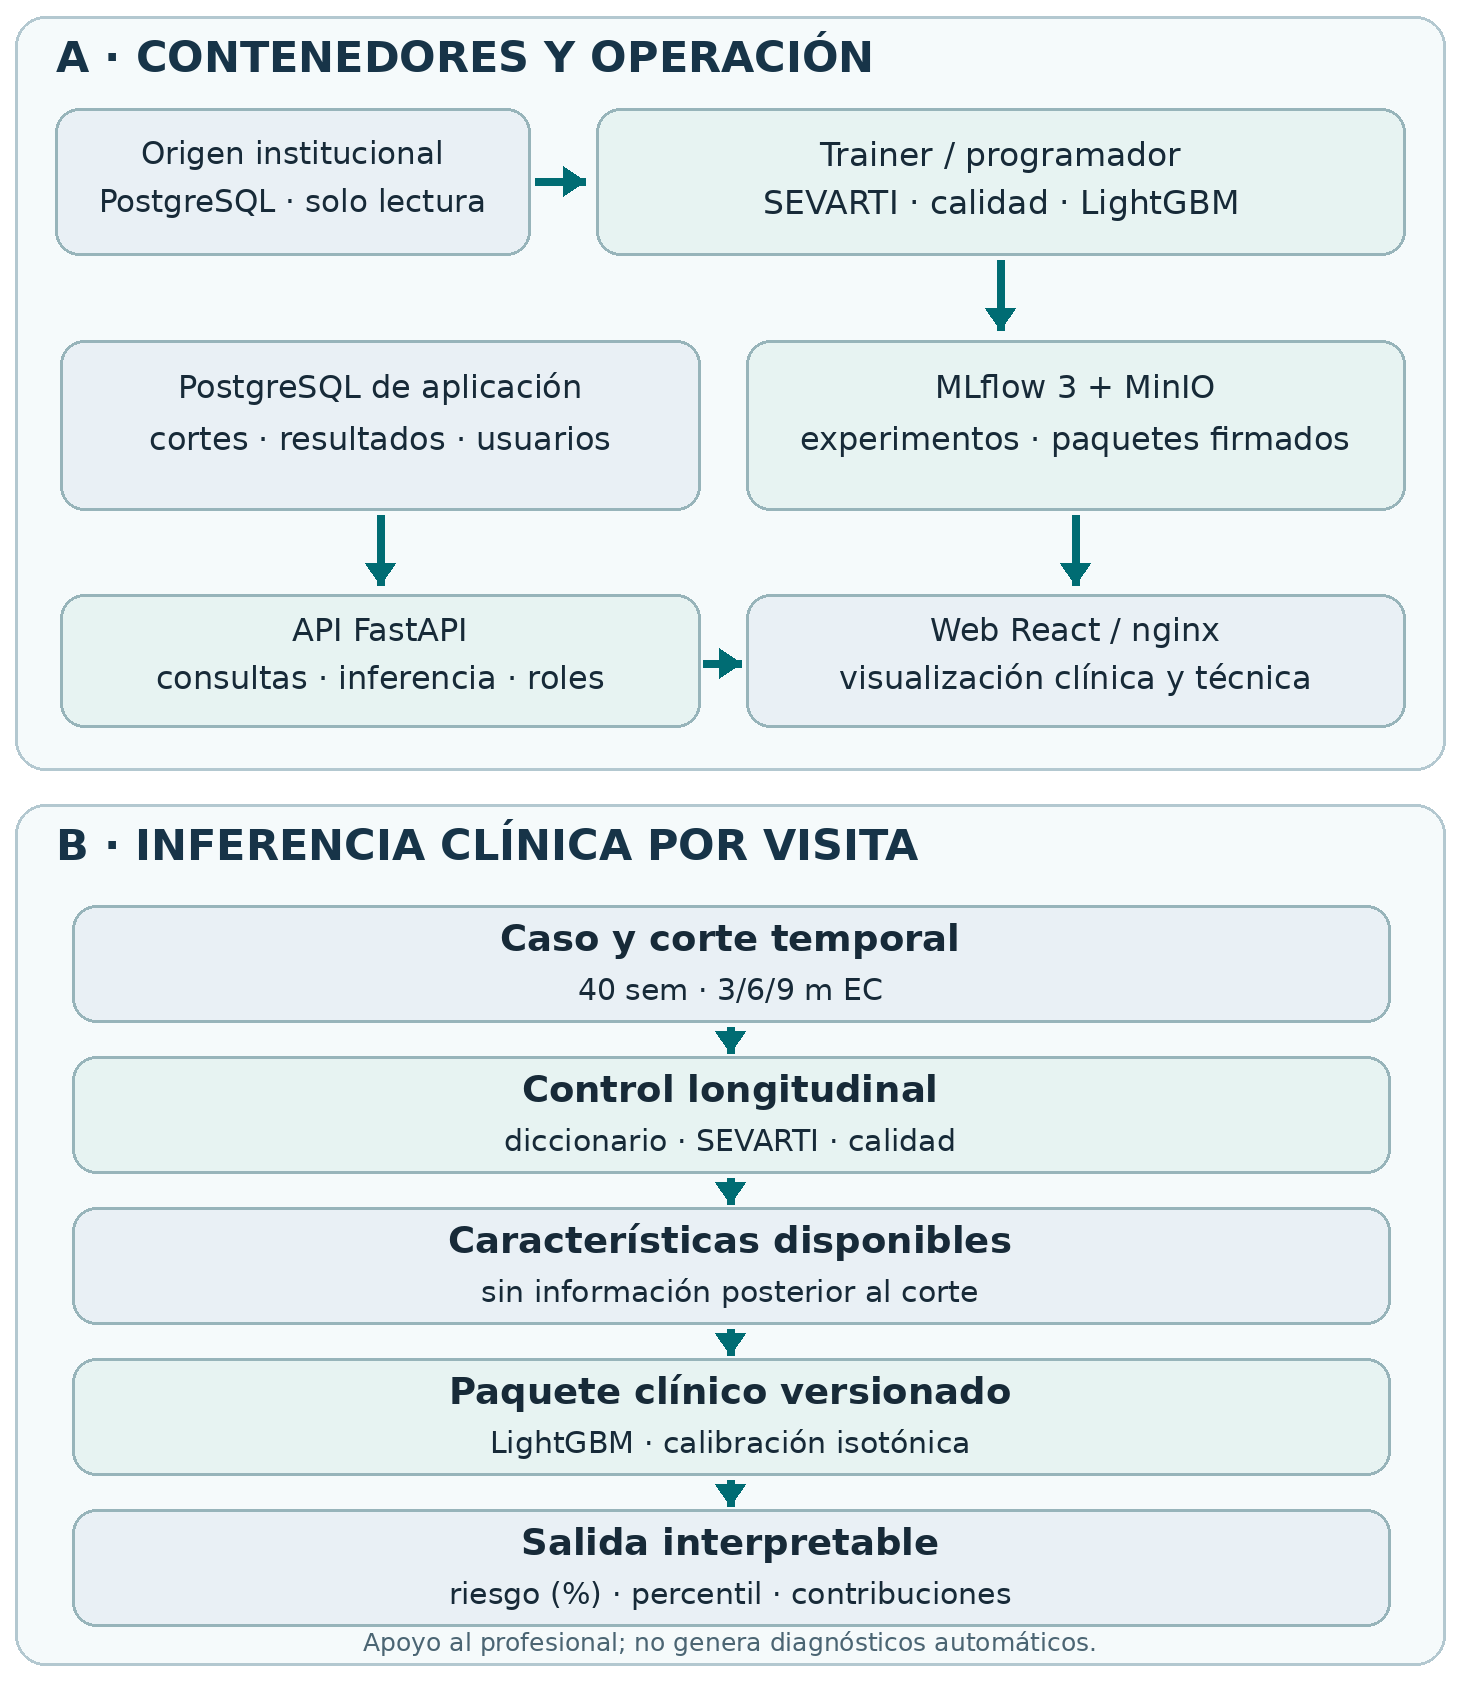
\includegraphics[width=\columnwidth]{figuras/image2.png}
\caption{Esquemas resumidos de (A) contenedores y operación y (B) inferencia por visita; elaboración propia.}
\label{fig:2}
\end{figure}

Buscamos que el profesional pueda consultar resultados sin entrar en los detalles del entrenamiento. Por eso la interfaz reúne seguimiento clínico, selección y comparación de cohortes, ficha individual y estimación de riesgo, mientras que la revisión técnica y la administración tienen apartados separados. Cada paquete conserva la versión del modelo, el diccionario y el corte de datos. En el entorno institucional se trabaja con registros autorizados; para las demostraciones se utilizan ejemplos sintéticos y permisos diferenciados.

Cuando se calcula el riesgo de un niño, la aplicación toma la información disponible hasta la visita seleccionada, prepara su trayectoria y aplica el modelo correspondiente. El resultado puede incluir el riesgo estimado, el percentil y las explicaciones disponibles. Las estimaciones de grupos grandes se ejecutan en segundo plano, y los cálculos detallados por niño no se guardan automáticamente. Esta separación busca facilitar la consulta clínica sin perder el control sobre las operaciones técnicas.

La plataforma utiliza seis servicios principales: interfaz web con React, Vite y nginx; API con FastAPI y SQLAlchemy; procesos de entrenamiento con Python y LightGBM; PostgreSQL 16; MLflow 3 para registrar modelos, y MinIO para almacenar artefactos. Los servicios se ejecutan en contenedores Docker, desplegados con Coolify sobre infraestructura propia. Además de pruebas automáticas de Python y de la web, se verifican las firmas y los archivos de los paquetes antes de utilizarlos y se aplican permisos según el rol.
